\section{Local Planar Objects}
The form factor of very anisotropic particles with local planar
geometry can be shown to factorize (see, e.g. \cite{Porod1948})
into a cross-section form factor $P_\text{cs}(Q)$ for the shorter
dimensions and a shape factor $P'(Q)$ for the larger dimension:
\begin{align}
P_\text{planar}(Q) = P'(Q) P_\text{cs}(Q)
\end{align}

The factorization in the cross-section factor $P_\text{cs}(Q)$, which only depends on parameters describing the
inner structure of the layer with short dimensions and the shape factor $P'(Q)$, describing the overall shape in the larger dimension
has the big advantage when both the shorter dimension as well as the larger dimensions have a polydispersity.
In this case we do not end up with a double integral but rather a product of two integrals when both a short and a large
dimension have a polydispersity. This speeds up the numerical computation significantly. Therefore the following form factors
already have a polydispersity parameter included.

\subsection{Shape factors $P'(Q)$}
\label{subsubsect:ShapeFactor}
\hspace{1pt} \\
The shape form factor $P'(Q)$ are normalized for $Q\rightarrow 0$ on the squared surface area
$S$ ($\lim_{Q\rightarrow 0} P'(Q) = S^2$) and can be that of an infinitely thin disc,
spherical shell, elliptical shell, or cylindrical shell:
The shape factors are  accessible as a structure factor under \verb"[anisotropic obj.|P'(Q):local planar geometry|P'(Q) xxx]"
and using the monodisperse approximation. Actually these shape factors are foreseen to be used with the cross-section factors
available as form factors under \verb"[anisotropic obj.|Pcs(Q) for planar obj.|Pcs(Q) xxx]".
The shape factors are also available in combination with some cross-section factors as form factors
under \verb"[planar obj.]".
~\\

\subsubsection{Polydisperse infinitesimal thin discs}
\label{subsubsect:ThinDisc}
\hspace{1pt} \\
\begin{align}
P'_\text{disc}(Q,R) &=\frac{2\pi^2R^4}{(QR)^2} \left(1-\frac{\text{J}_1(2QR)}{QR}\right)
\end{align}
The polydispersity is included as a \texttt{LogNormal}-distribution from section \ref{sect:LogNormSD} by
\begin{align}
P'_\text{ThinDiscs}(Q,R,\sigma) &= \int_0^\infty \mathrm{LogNorm}(R',R,\sigma,1) P'_\text{disc}(Q,R') \; \mathrm{d}R'
\end{align}

\subsubsection{Infinitesimal thin spherical shell}
\label{subsubsect:ThinSphShell}
\hspace{1pt} \\
\begin{align}
P'_\text{sph. shell}(Q,R) &= \left(4\pi R^2\frac{\sin QR}{QR}\right)^2 \\
\end{align}

\subsubsection{Infinitesimal thin elliptical shell}
\label{subsubsect:ThinEllShell}
\hspace{1pt} \\
\begin{align}
P'_\text{ell. shell}(Q,R,\epsilon) &= S^2 \int_0^{\pi/2}
\left(\,\frac{\sin\left( QR\sqrt{\sin^2\alpha+\epsilon^2\cos^2\alpha}\right)}{QR\sqrt{\sin^2\alpha+\epsilon^2\cos^2\alpha}}\right)^2 \sin(\alpha) \;\mathrm{d}\alpha \\
\mbox{with } \quad S &=
\begin{cases}
4\pi R^2 & \mbox{for } \epsilon = 1 \\
2 \pi R^2 \left(1+\epsilon \frac{\arccos(1/\epsilon)}{\tan\left(\arccos(1/\epsilon)\right)} \right)& \mbox{for } \epsilon > 1 \\
2 \pi R^2 \left(1+\epsilon \frac{\mathrm{arctanh}\left(\sin(\arccos(\epsilon))\right)}{\sin\left(\arccos(\epsilon)\right)} \right)& \mbox{for } \epsilon < 1
\end{cases}
\end{align}

\subsubsection{Infinitesimal thin cylindrical shell}
\label{subsubsect:ThinCylShell}
\hspace{1pt} \\
\begin{multline}
P'_\text{closed cyl. sh.}(Q,R,H) = \int_0^{\pi/2}\left(2 \pi R^2+2 \pi R H\right)^2 \\
\left(\frac{R}{R+H}
\frac{2\mathrm{J}_1\left(QR\sin(\alpha)\right)}{QR\sin(\alpha)} \cos(QH\cos(\alpha)/2) + \right.\\
\left.
\frac{H}{R+H}\mathrm{J}_0(QR\sin{\alpha})\frac{\sin(QH\cos(\alpha)/2)}{QH\cos(\alpha)/2}\right)^2\sin(\alpha) \; \mathrm{d}\alpha
\end{multline}



\clearpage

\subsection{Cross-section form factors $P_\text{cs}(Q)$}

\subsubsection{homogeneousXS}
\label{sect:homogeneousXS}
\hspace{1pt} \\
\begin{figure}[htb]
\begin{center}
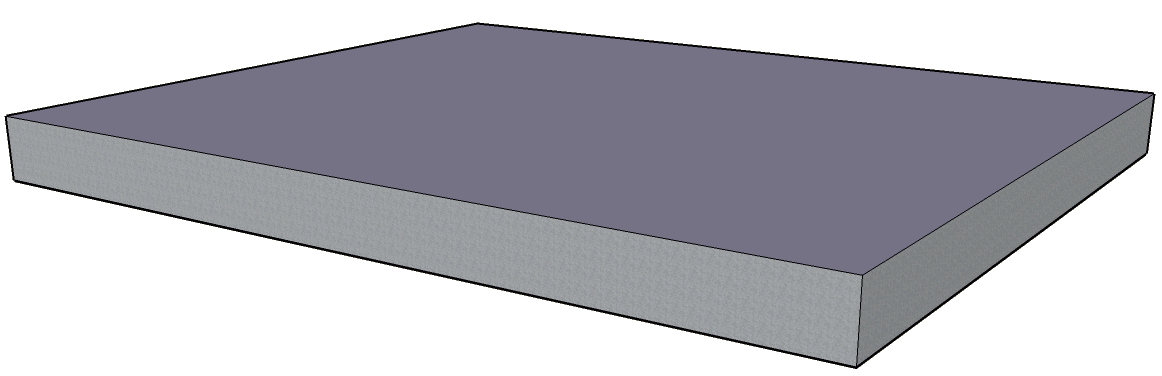
\includegraphics[width=0.6\textwidth,height=0.4\textwidth]{planarHomo.png}
\end{center}
\caption{Planar object with homogeneous cross-section.}
\label{fig:planarHomo}
\end{figure}

\begin{align}
P_\text{cs}(Q,\eta,L) = \left( \eta L\frac{\sin(QL/2)}{QL/2}\right)^2
\end{align}
%%%%%%%%%%%%%%%%%%%%%%%%%%%%%%%%%%%%%%%%%%%%%%%%%%%%%%%%%%%%%%%%%%%%%

\clearpage
\subsection{TwoInfinitelyThinPlates}
\label{sect:TwoInfinitelyThinPlates}
\hspace{1pt} \\
\begin{figure}[htb]
\begin{center}
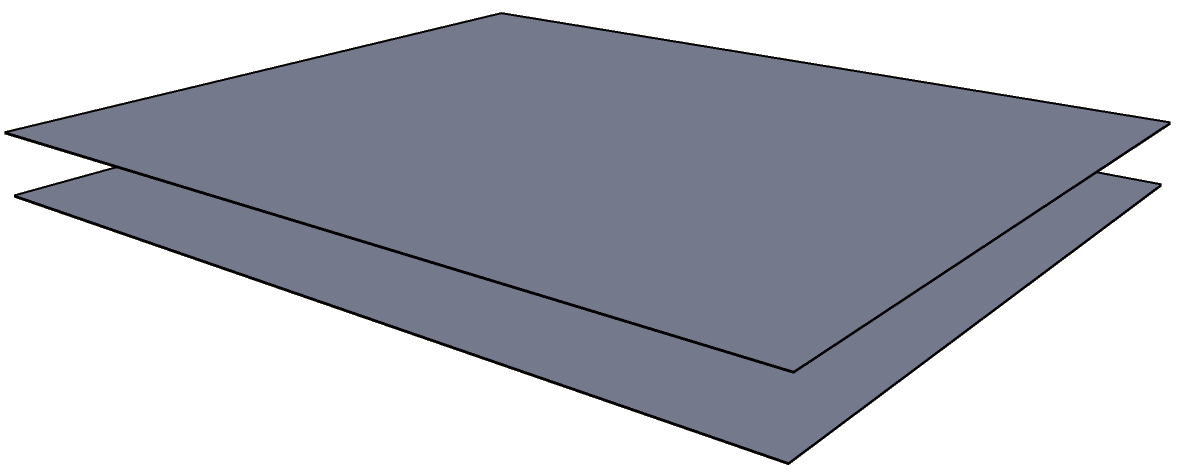
\includegraphics[width=0.6\textwidth,height=0.4\textwidth]{planar2thin.png}
\end{center}
\caption{planar2thin.}
\label{fig:planar2thin}
\end{figure}
\begin{align}
P_\text{cs}(Q,\eta,L) = \eta^2 \cos^2(QL/2)
\end{align}


%%%%%%%%%%%%%%%%%%%%%%%%%%%%%%%%%%%%%%%%%%%%%%%%%%%%%%%%%%%%%%%%%%%%%
\clearpage
\subsection{LayeredCentroSymmetricXS}
\label{sect:LayeredCentroSymmetricXS}
~\\

\begin{figure}[htb]
\begin{center}
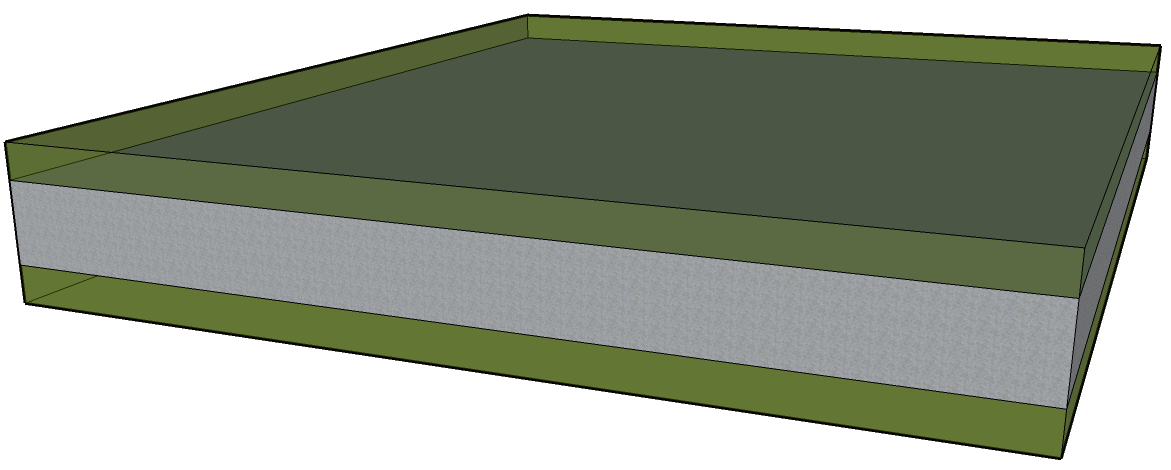
\includegraphics[width=0.6\textwidth,height=0.4\textwidth]{planar2centrosymm.png}
\end{center}
\caption{planar2centrosymHomo.}
\label{fig:planar2centrosymm}
\end{figure}
A layered centro symmetric cross-section structure with outer
thickness $L_\text{out}$ and a core of thickness $L_c$, where the
core and the outer part have the scattering lengths density
$\eta_\text{out}$ and $\eta_c$, respectively, has
\begin{align}
P_\text{cs}(Q,\eta_\text{out},L_\text{out},\eta_c,L_c)
= \Biggl( & \frac{\eta_\text{out}L_\text{out}\sin\left(\frac{QL_\text{out}}{2}\right)}{QL_\text{out}/2} \\
&-  \frac{(\eta_\text{out}-\eta_c)L_c\sin\left(\frac{QL_c}{2}\right)}{QL_c/2}\Biggr)^2 \nonumber
\end{align}

%%%%%%%%%%%%%%%%%%%%%%%%%%%%%%%%%%%%%%%%%%%%%%%%%%%%%%%%%%%%%%%%%%%%%%%%%

\clearpage
\subsection{BiLayerGauss \cite{Pabst2000}}
\label{sect:BiLayerGauss}
~\\
\begin{figure}[htb]
\begin{center}
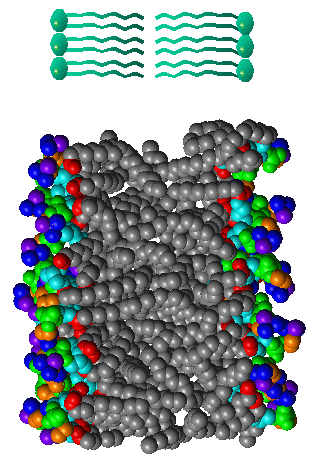
\includegraphics[width=0.4\textwidth,height=0.5\textwidth]{BiLayers.png}
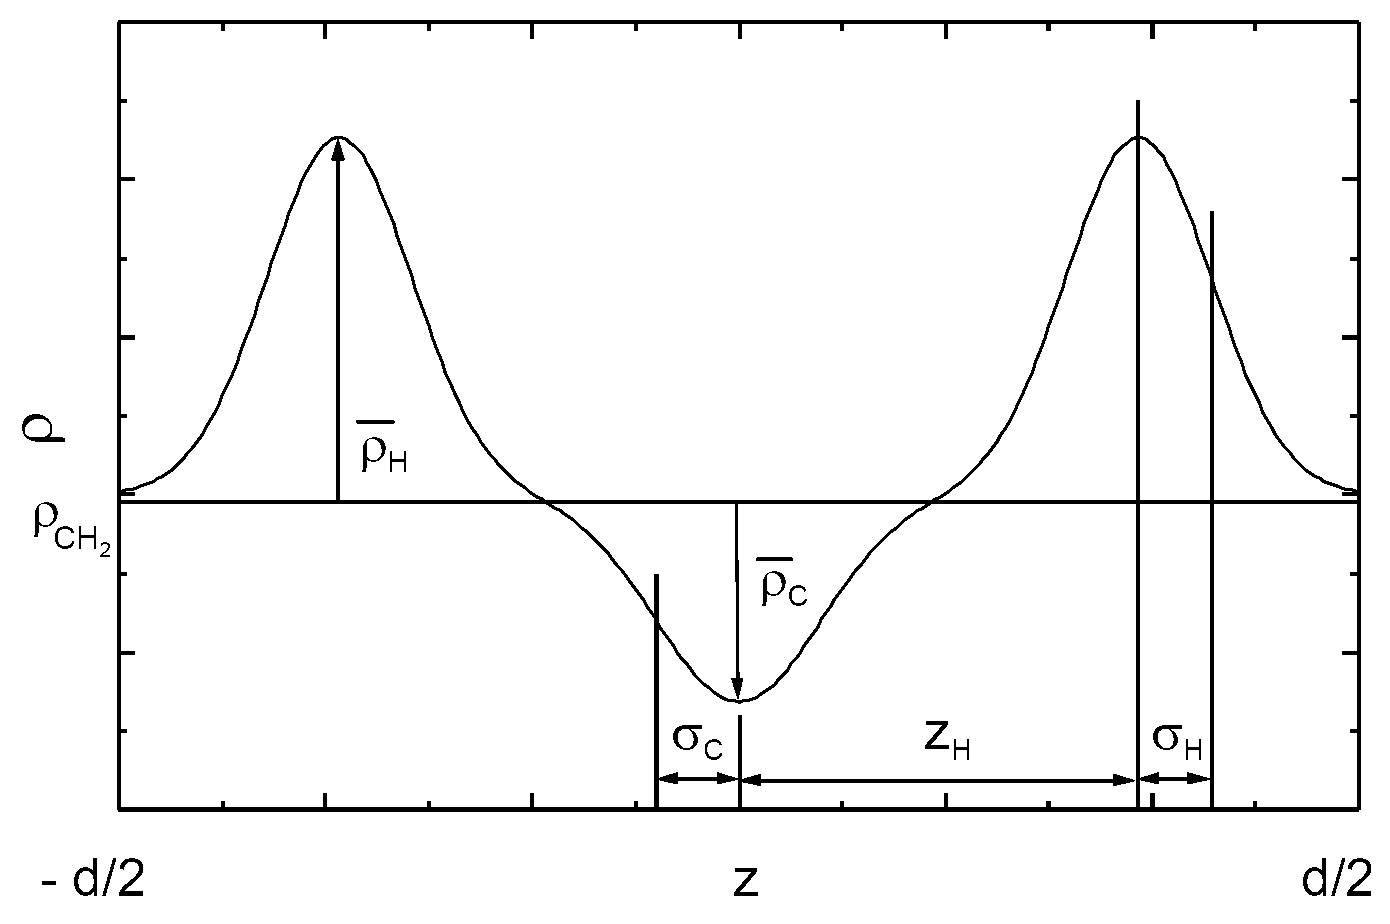
\includegraphics[width=0.5\textwidth,height=0.4\textwidth]{bilayerprofile.png}
\end{center}
\caption{bilayerprof.}
\label{fig:bilayerprof}
\end{figure}

\begin{align}
   u_\text{out}  &= Q\sigma_\text{out} \\
   u_\text{core} &= Q\sigma_\text{core} \\
   F_\text{out}  &= \sqrt{2\pi}\sigma_\text{out}  b_\text{out}  \exp(-u_\text{out}^2/2) \cos(Qt/2) \\
   F_\text{core} &= \sqrt{2\pi}\sigma_\text{core} b_\text{core} \exp(-u_\text{core}^2/2)  \\
   P_\text{cs}   &=(F_\text{core}+2 F_\text{out})^2
\end{align}
